\documentclass[12pt]{article}

\usepackage[a4paper,margin=1in]{geometry}
\usepackage{setspace}
\usepackage{microtype}
\usepackage{graphicx}
\usepackage{booktabs}
\usepackage{array}
\usepackage{enumitem}
\usepackage{hyperref}
\usepackage{caption}
\usepackage{float}
\usepackage{tikz}
\usetikzlibrary{arrows.meta,positioning,shapes.geometric,shapes.misc}

\hypersetup{
  colorlinks=true,
  linkcolor=black,
  urlcolor=blue,
  citecolor=black
}

\setstretch{1.15}
\setlist{nosep}
\raggedbottom

\title{SignalShift: A Reproducible Data-Science Pipeline for Review Sentiment Classification and Issue Discovery}
\author{%
\textbf{Course:} MCA (Master of Computer Applications)\\
\textbf{Subject Code:} PAMCA602\\
\textbf{Subject Title:} Python for Data Science\\
\textbf{Slot:} B2 + TB2\\
\textbf{Class No:} VL2025260502657\\
\textbf{Semester:} Winter Semester (2025--2026)\\[6pt]
\begin{tabular}{@{}r l l@{}}
\toprule
\textbf{Serial No.} & \textbf{Register No.} & \textbf{Name} \\
\midrule
1 & 25MCA0086 & Meghna \\
2 & 25MCA0187 & Subarta Ghosh \\
\bottomrule
\end{tabular}%
}
\date{}

\begin{document}
\maketitle

\begin{abstract}
User-generated reviews contain valuable signals about user satisfaction and recurring product issues, but raw review corpora are noisy, large, and difficult to summarize reliably. This paper describes a practical data-science pipeline that converts unstructured review text into (i) supervised sentiment labels for KPI monitoring and (ii) ranked issue categories for root-cause analysis. The workflow begins with data validation and text normalization to produce a cleaned training dataset. Next, a TF--IDF vectorizer is fitted once on curated training text to define a stable feature space and then reused for all downstream transformations. Sentiment labels are derived from existing rating metadata (weak supervision), enabling scalable supervised learning without manual annotation. A linear classifier (logistic regression) is trained on TF--IDF features and evaluated using a held-out split, producing standard classification metrics such as accuracy and per-class precision/recall. In parallel, the pipeline generates semantic embeddings for a curated issue taxonomy using a sentence-embedding model. New reviews can then be matched to issue categories by vector similarity, and the results aggregated to produce top-issue rankings and representative examples.

The key design principle is artifact reproducibility: the vectorizer and model are persisted and reused, preventing feature mismatch and making retraining deterministic. The resulting system provides an interpretable baseline for sentiment classification and an actionable framework for discovering and prioritizing product issues from text at scale.
\end{abstract}

\section*{Block Diagram (Pipeline Overview)}
\begin{figure}[H]
  \centering
  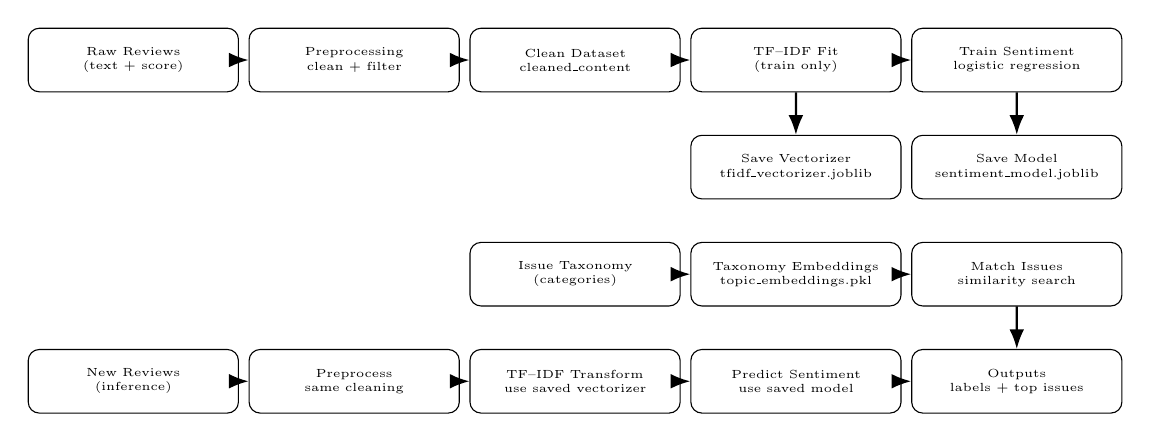
\begin{tikzpicture}[
      x=1cm,
      y=1cm,
      scale=0.85,
      transform shape,
      font=\tiny,
      box/.style={draw, rounded corners, align=center, text width=3.0cm, minimum height=0.95cm, inner sep=2pt},
      arrow/.style={-{Latex[length=2.5mm]}, thick}
  ]
  % Fixed grid (prevents overlap) and compact text (cleaner)
  % Columns: 0, 3.3, 6.6, 9.9, 13.2
  % Rows: training=0, artifacts=-1.6, taxonomy=-3.2, inference=-4.8

  % --- Training pipeline ---
  \node[box] (raw)   at (0,0)    {Raw Reviews\\(text + score)};
  \node[box] (prep)  at (3.3,0)  {Preprocessing\\clean + filter};
  \node[box] (clean) at (6.6,0)  {Clean Dataset\\cleaned\_content};
  \node[box] (tfidf) at (9.9,0)  {TF--IDF Fit\\(train only)};
  \node[box] (train) at (13.2,0) {Train Sentiment\\logistic regression};

  \node[box] (vecsave)   at (9.9,-1.6)  {Save Vectorizer\\tfidf\_vectorizer.joblib};
  \node[box] (modelsave) at (13.2,-1.6) {Save Model\\sentiment\_model.joblib};

  % --- Issue taxonomy ---
  \node[box] (tax)    at (6.6,-3.2)  {Issue Taxonomy\\(categories)};
  \node[box] (emb)    at (9.9,-3.2)  {Taxonomy Embeddings\\topic\_embeddings.pkl};
  \node[box] (match)  at (13.2,-3.2) {Match Issues\\similarity search};

  % --- Inference pipeline ---
  \node[box] (new)     at (0,-4.8)   {New Reviews\\(inference)};
  \node[box] (prep2)   at (3.3,-4.8) {Preprocess\\same cleaning};
  \node[box] (xform)   at (6.6,-4.8) {TF--IDF Transform\\use saved vectorizer};
  \node[box] (pred)    at (9.9,-4.8) {Predict Sentiment\\use saved model};
  \node[box] (out)     at (13.2,-4.8){Outputs\\labels + top issues};

  % --- Arrows ---
  \draw[arrow] (raw) -- (prep);
  \draw[arrow] (prep) -- (clean);
  \draw[arrow] (clean) -- (tfidf);
  \draw[arrow] (tfidf) -- (train);

  \draw[arrow] (tfidf) -- (vecsave);
  \draw[arrow] (train) -- (modelsave);

  \draw[arrow] (tax) -- (emb);
  \draw[arrow] (emb) -- (match);

  \draw[arrow] (new) -- (prep2);
  \draw[arrow] (prep2) -- (xform);
  \draw[arrow] (xform) -- (pred);
  \draw[arrow] (pred) -- (out);

  % Use taxonomy embeddings during inference
  \draw[arrow] (match) -- (out);

  \end{tikzpicture}
  \caption{Block diagram of the data-science pipeline: training creates reusable artifacts (vectorizer + model) and inference reuses them while performing issue discovery using taxonomy embeddings.}
\end{figure}

\section{Identified Machine Learning / Data Science Project Description}
\subsection{Problem Statement}
Online product reviews provide high-volume feedback about user experience, failures, and feature requests. Stakeholders typically need two types of signals: (1) a quantitative indicator of satisfaction (sentiment) and (2) a qualitative summary of recurring issues (themes) to guide prioritization. Manual reading does not scale; naive keyword counting can miss paraphrases and synonyms; and inconsistent preprocessing can cause unstable features and misleading results.

This project addresses two complementary tasks on review text:
\begin{enumerate}[label=(\arabic*)]
  \item \textbf{Sentiment classification (supervised learning):} classify each review as \emph{positive} or \emph{negative}.
  \item \textbf{Issue discovery and ranking (semantic matching):} assign each review to a curated issue taxonomy using semantic embeddings, then aggregate assignments to produce top-issue rankings.
\end{enumerate}

\subsection{Data and Labeling Strategy}
The dataset consists of a large CSV of reviews containing at minimum the review text and a rating score. The rating score is used as a weak supervision signal: low ratings are mapped to \emph{negative} sentiment and higher ratings to \emph{positive} sentiment. This strategy avoids expensive manual annotation while still creating a large labeled set suitable for classical supervised learning.

While weak labels can be imperfect (e.g., neutral ratings with mixed language), they are effective for building a baseline sentiment system and provide consistent targets for evaluation and iteration. The pipeline reports label distribution to help validate class balance.

\subsection{Text Preprocessing}
Text preprocessing improves robustness by removing invalid rows and normalizing content. The pipeline:
\begin{itemize}
  \item drops rows with missing review text,
  \item drops empty/whitespace-only strings,
  \item applies a text cleaning function to produce \texttt{cleaned\_content}, and
  \item removes rows that become empty after cleaning.
\end{itemize}

This produces a stable training corpus and reduces downstream errors during vectorization and model training.

\subsection{Feature Engineering with TF--IDF}
To model text with classical machine learning, reviews must be converted into numeric vectors. TF--IDF (term frequency--inverse document frequency) is used because it is efficient, widely validated for text classification, and performs well on review-length documents. The implementation uses a capped vocabulary and includes both unigrams and bigrams to capture informative phrases (e.g., \emph{customer service}, \emph{video quality}).

A critical design choice is that TF--IDF is \textbf{fitted exactly once on the curated training corpus}. Fitting learns the vocabulary and IDF weights that define the feature space. Persisting the fitted vectorizer ensures that all later transformations (training and inference) share identical features.

\subsection{Sentiment Modeling with Logistic Regression}
The sentiment classifier is a logistic regression model trained on sparse TF--IDF vectors. Logistic regression is a strong baseline for text classification due to its scalability, good performance on high-dimensional sparse features, and interpretability. The model is evaluated on a held-out test split to estimate generalization. Standard metrics (accuracy and per-class precision/recall) are reported.

\subsection{Issue Taxonomy and Semantic Embeddings}
In addition to sentiment, the project builds an \emph{issue discovery} layer. A curated set of issue labels/descriptions (taxonomy) is encoded into dense vectors using a sentence embedding model. Reviews can be embedded and matched to the closest taxonomy vector by similarity. Aggregating matches provides ranked issue counts and representative examples.

This hybrid approach yields both a numerical sentiment KPI and an actionable list of recurring problems.

\section{Implementation Description and Results (No Code)}
\subsection{Implementation Structure}
The pipeline is implemented as four sequential steps that produce reusable artifacts:
\begin{itemize}
  \item \textbf{Step 01: Preprocessing} produces a cleaned dataset with \texttt{cleaned\_content}.
  \item \textbf{Step 02: Vectorization} fits TF--IDF on training text and persists the vectorizer artifact.
  \item \textbf{Step 03: Sentiment Training} loads the persisted vectorizer, transforms text, trains logistic regression, evaluates it, and persists the classifier artifact.
  \item \textbf{Step 04: Issue Embeddings} encodes the issue taxonomy and persists taxonomy embeddings for similarity matching.
\end{itemize}

The design follows the principle \emph{train once, reuse everywhere}. In particular, Step 03 uses \emph{transform} with the already-fitted TF--IDF vectorizer rather than refitting. This avoids feature mismatch and makes experiments reproducible.

For deployment and demonstration, the trained artifacts can be served through a lightweight API layer (implemented using FastAPI) so the same preprocessing and inference steps are accessible programmatically.

\subsection{Training Procedure}
After preprocessing, the TF--IDF vectorizer is fitted on the cleaned training corpus. The sentiment targets are derived from rating score. The training matrix is built by applying the saved vectorizer to the cleaned text. The classifier is trained on a training split and evaluated on a held-out split.

\subsection{Evaluation Method}
The system reports:
\begin{itemize}
  \item sentiment class distribution to check label balance,
  \item accuracy on the held-out split, and
  \item a per-class classification report (precision, recall, F1-score).
\end{itemize}

These metrics provide a transparent baseline and support iterative improvement (e.g., refining cleaning, adjusting TF--IDF settings, or improving label mapping).

\subsection{Result Snapshot}
Figure~\ref{fig:frontend-snapshot} shows a sample results view generated from the pipeline outputs.

\begin{figure}[H]
  \centering
  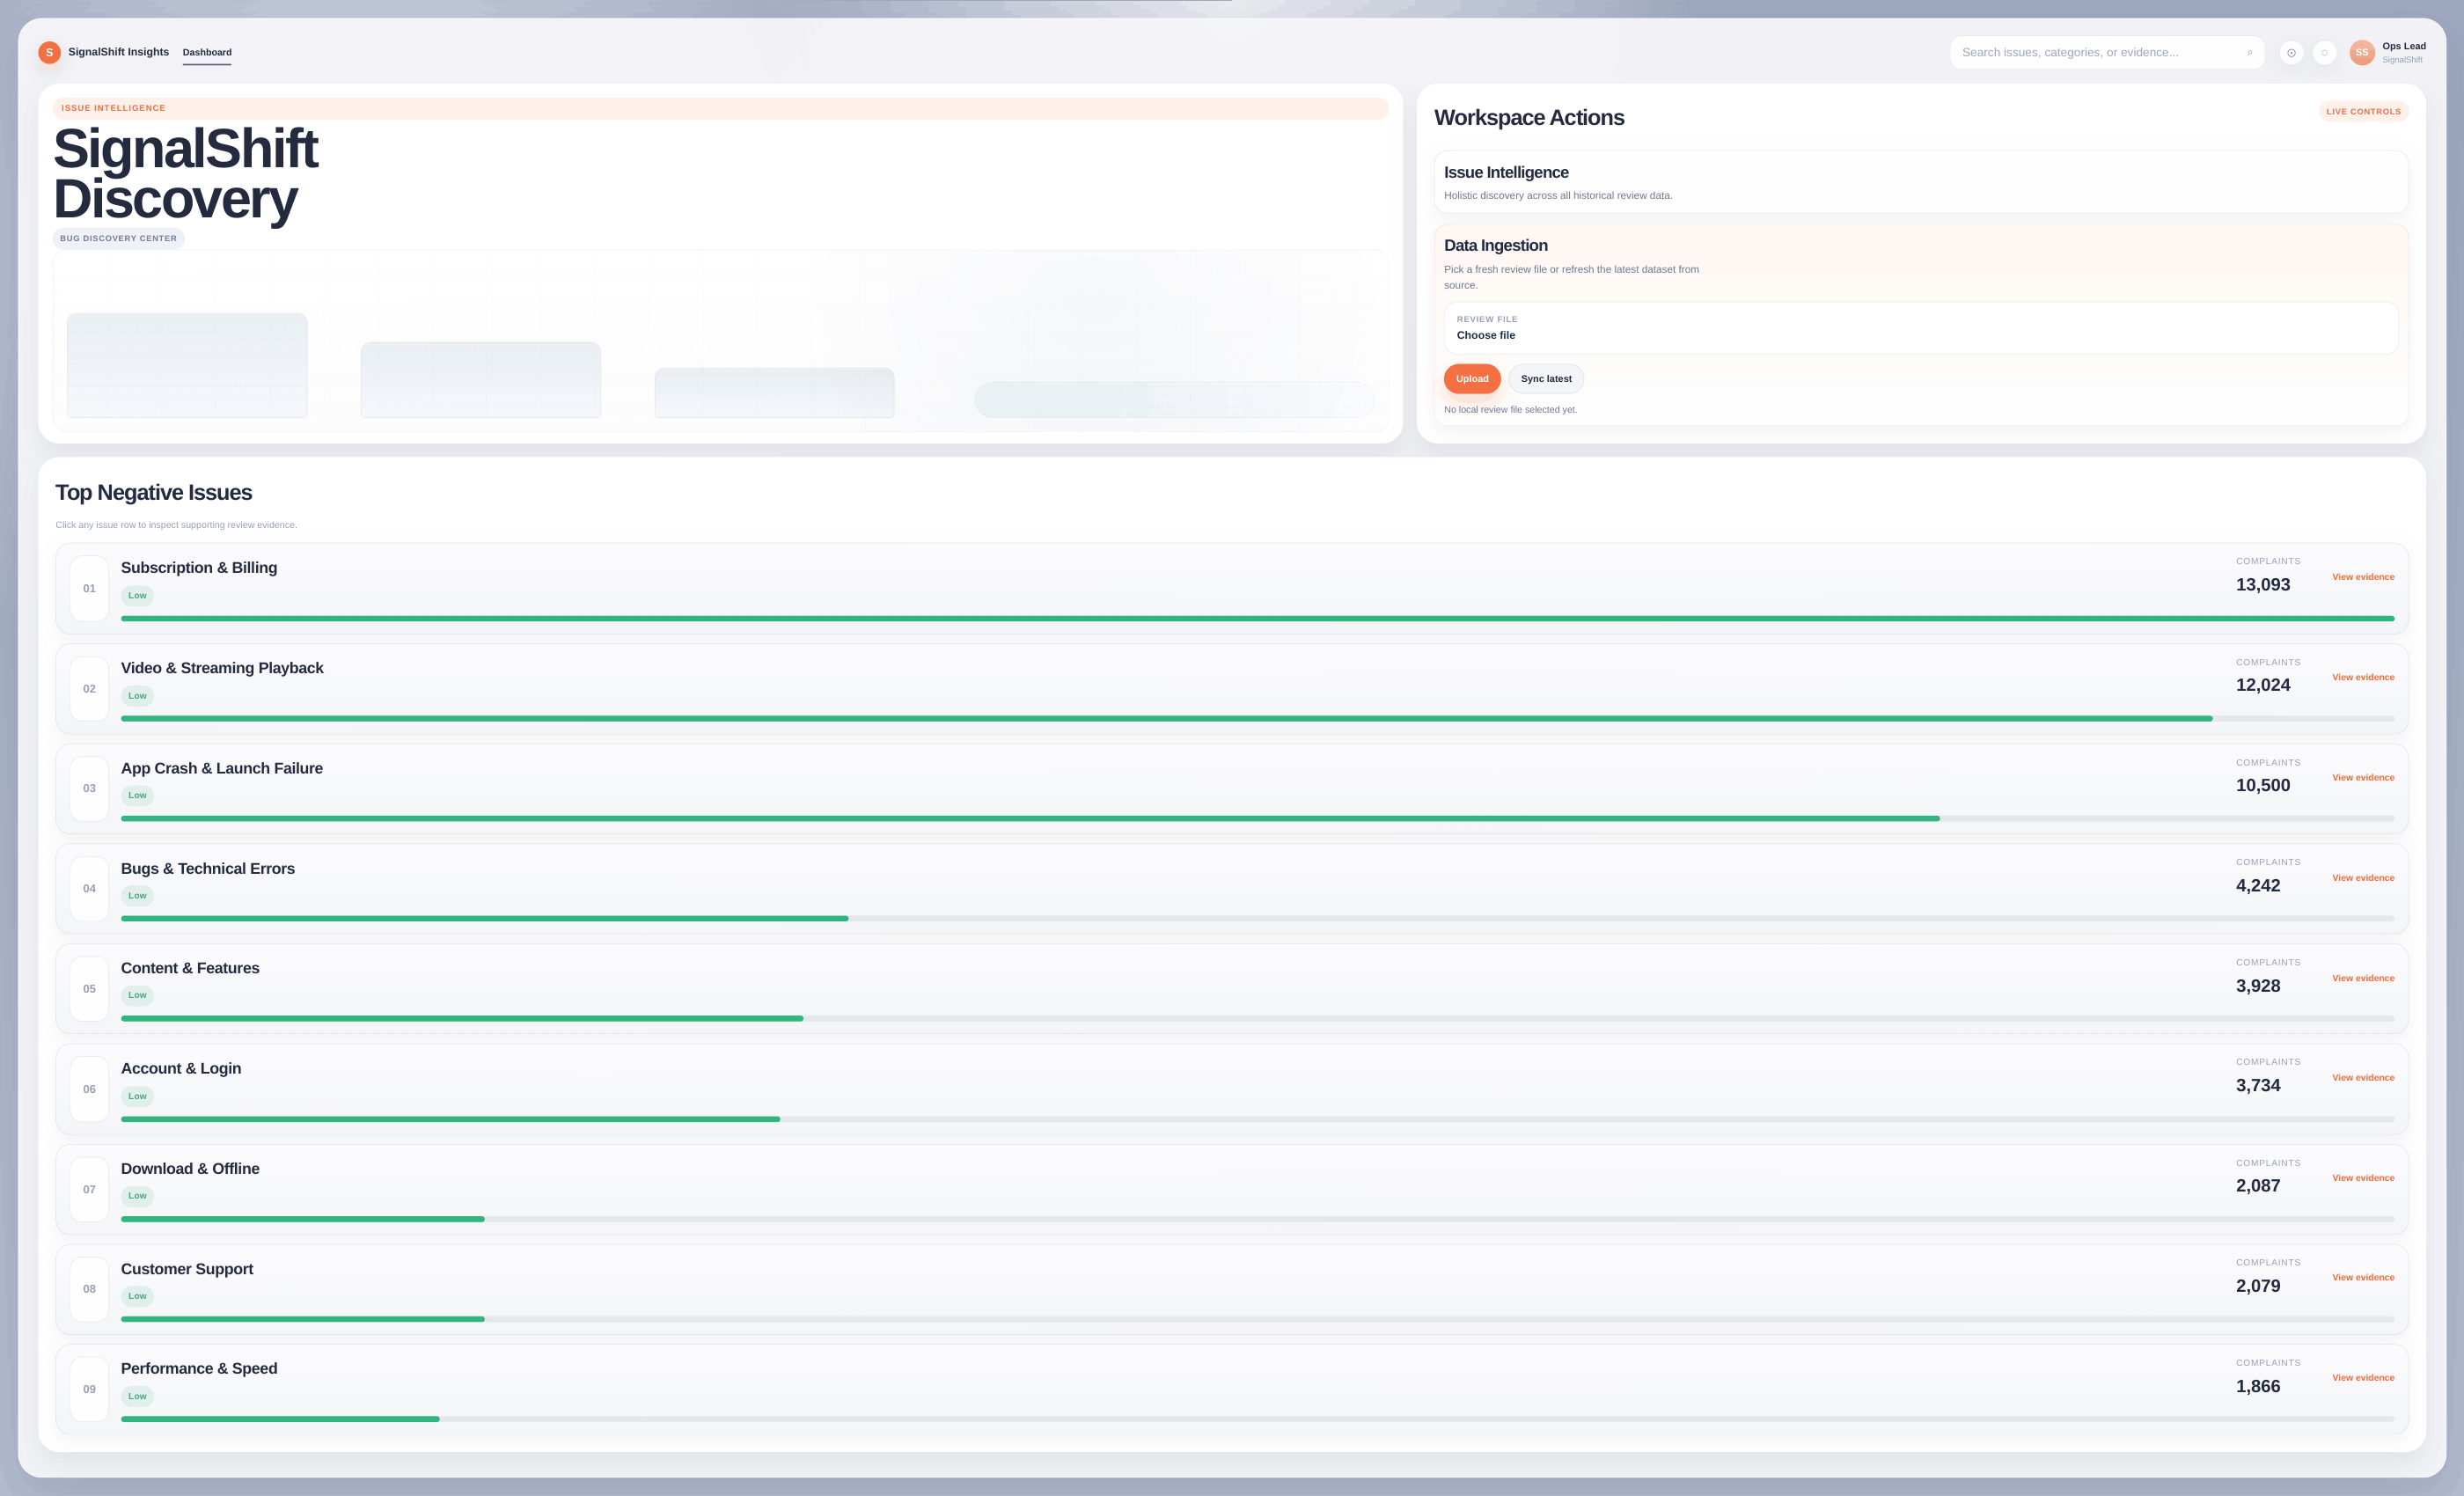
\includegraphics[width=0.95\linewidth]{frontend1-1.png}
  \caption{Result snapshot (example view of the produced analysis).}
  \label{fig:frontend-snapshot}
\end{figure}

\subsection{Issue Discovery Outputs}
The issue discovery component produces an issue-level summary by assigning reviews to the closest taxonomy category via embedding similarity. The outputs include:
\begin{itemize}
  \item a ranked list of top issue categories,
  \item counts per category, and
  \item representative review excerpts per issue (for qualitative validation).
\end{itemize}

This directly supports root-cause analysis: teams can see which complaints are most prevalent and track changes over time.

\subsection{Reproducible Artifacts}
The persisted artifacts enable consistent reuse:
\begin{itemize}
  \item a saved TF--IDF vectorizer defines the feature space,
  \item a saved sentiment model performs predictions on new text, and
  \item saved issue embeddings support efficient semantic matching.
\end{itemize}

This separation of concerns reduces pipeline redundancy and helps ensure the same transformations are applied during training and inference.

\section{Conclusion and References}
\subsection{Conclusion}
This paper presented a modular data-science pipeline for extracting sentiment and prioritized issue themes from review text. The approach combines robust preprocessing, TF--IDF feature extraction, and a logistic regression sentiment classifier with a semantic issue discovery layer based on sentence embeddings. Persisted artifacts (vectorizer, classifier, and taxonomy embeddings) enable reproducible training and consistent inference without feature mismatch. The result is an interpretable baseline suitable for review monitoring, satisfaction KPIs, and actionable issue prioritization.

\subsection*{References (10)}
\begin{thebibliography}{10}
\bibitem{salton1988} G.~Salton and C.~Buckley, ``Term-weighting approaches in automatic text retrieval,'' \emph{Information Processing \& Management}, vol.~24, no.~5, pp.~513--523, 1988.

\bibitem{manning2008} C.~D.~Manning, P.~Raghavan, and H.~Sch\"utze, \emph{Introduction to Information Retrieval}. Cambridge University Press, 2008.

\bibitem{pang2002} B.~Pang, L.~Lee, and S.~Vaithyanathan, ``Thumbs up? Sentiment classification using machine learning techniques,'' in \emph{Proceedings of EMNLP}, 2002.

\bibitem{joachims1998} T.~Joachims, ``Text categorization with Support Vector Machines: Learning with many relevant features,'' in \emph{Proceedings of ECML}, 1998.

\bibitem{sebastiani2002} F.~Sebastiani, ``Machine learning in automated text categorization,'' \emph{ACM Computing Surveys}, vol.~34, no.~1, pp.~1--47, 2002.

\bibitem{devlin2019} J.~Devlin, M.-W.~Chang, K.~Lee, and K.~Toutanova, ``BERT: Pre-training of deep bidirectional transformers for language understanding,'' in \emph{Proceedings of NAACL-HLT}, 2019.

\bibitem{reimers2019} N.~Reimers and I.~Gurevych, ``Sentence-BERT: Sentence embeddings using Siamese BERT-networks,'' in \emph{Proceedings of EMNLP-IJCNLP}, 2019.

\bibitem{mikolov2013} T.~Mikolov, K.~Chen, G.~Corrado, and J.~Dean, ``Efficient estimation of word representations in vector space,'' in \emph{ICLR Workshop}, 2013.

\bibitem{kowsari2019} K.~Kowsari, K.~Jafari~Meimandi, M.~Heidarysafa, S.~Mendu, L.~Barnes, and D.~Brown, ``Text classification algorithms: A survey,'' \emph{Information}, vol.~10, no.~4, p.~150, 2019.

\bibitem{aggarwal2012} C.~C.~Aggarwal and C.~Zhai, ``A survey of text classification algorithms,'' in \emph{Mining Text Data}. Springer, 2012.
\end{thebibliography}

\end{document}
